\documentclass{article}
\usepackage{listings}
\usepackage{xcolor}
\usepackage{graphicx}
\usepackage{float} 
\title{Software Assignment Report}
\author{Saketh Ram Kumar Dondapati}
\date{\today}

\definecolor{codebg}{RGB}{240,240,240}
\lstset{
    backgroundcolor=\color{codebg},
    basicstyle=\footnotesize\ttfamily,
    breaklines=true,
    keywordstyle=\color{blue},
    stringstyle=\color{orange},
    commentstyle=\color{gray},
    numbers=left,
    numberstyle=\tiny\color{gray},
    stepnumber=1,
    numbersep=5pt,
    captionpos=b,
    frame=tb
}

\begin{document}
\maketitle

\section{Introduction}
This report presents an implementation of a simple music player using the Pygame library. The program allows users to play, pause, skip songs, and shuffle the song list.

\section{Code Explanation}
The code consists of several components, each responsible for a specific functionality. Let's go through them step by step:

\subsection{Initializing Pygame and Audio Settings}
The Pygame library is initialized, along with the audio settings. The width and height of the game window are set, and the volume is configured.

\subsection{Loading Assets}
The necessary images for buttons and backgrounds are loaded using the \texttt{pygame.image.load} function and stored in variables for later use.

\subsection{Button Class}
A \texttt{Button} class is defined to represent clickable buttons in the user interface. It has attributes for position, image, and a method for drawing the button on the screen.

\subsection{Shuffle Function}
The \texttt{shuffle} function takes a list of songs as input and shuffles them randomly using the \texttt{numpy.random.choice} function. It returns the shuffled song list.

\subsection{Main Function}
The \texttt{main} function is the entry point of the program. It initializes variables, sets up the GUI elements, and enters the main event loop. The event loop handles user input and updates the display accordingly.

\subsection{Event Handling}
Within the event loop, various events are handled, such as button clicks, song changes, and program termination. The user's mouse position is obtained using the \texttt{pygame.mouse.get\_pos} function, and button clicks are detected by checking if the mouse position falls within the button's hitbox.
\section{Code Listing}
Below is the complete Python code for the program:

\lstinputlisting[language=Python]{main.py}

\begin{figure}[ht]
        \centering
        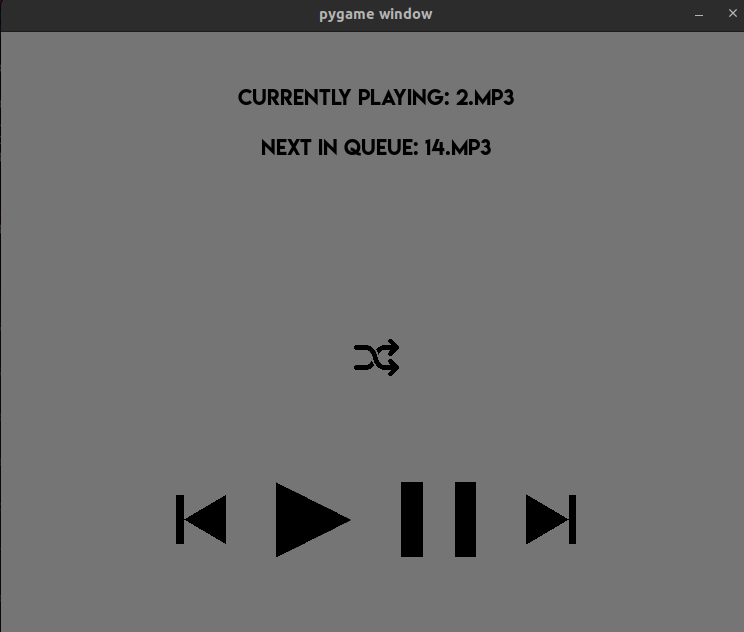
\includegraphics[width=0.8\linewidth]{GUI.png}
        \caption{Image of the GUI player}
        \label{fig:view}
\end{figure}

\section{Conclusion}
The implemented music player provides basic functionalities for playing, pausing, skipping songs, and shuffling the playlist. It serves as a starting point for further enhancements and customization.

\end{document}
